
\chapter{Aging in the Two-Dimensional Random Field Ising Model}
\label{chap-rfim}
The work in this chapter is motivated by the experimental study of antiferromagnet CoO polycrystalline films in Sergei Urazhdin's group \cite{ma2016prb}. In the experimental findings, glassy dynamics and non-Neel-Arrhenius aging has been discovered. In this computational study, a Monte Carlo simulation using the Random Field Ising Model (RFIM) is proposed to explain and understand the experimental findings.

This chapter first introduces RFIM and its connection with the experiment. Then the details of Monte Carlo simulations are described, and the choices of parameters are discussed. All the results from simulations  are shown in the third section (Sec. \ref{sec:rfim-results}). Finally, we conclude this chapter with interesting findings and discussions.
 
\section{Random Field Ising Model and experiments }
\label{sec:rfim-model}
As introduced in Sec. \ref{sec:intro-rfim}, the RFIM has been extensively utilized for modeling diluted antiferromagnets \cite{fernandez1988random}, impure substrates \cite{villain1982commensurate}, and magnetic alloys \cite{fisher1988theory}. The experimental system to simulate in this work is the polycrystalline films of antiferromagnet CoO \cite{ma2016prb}. It has 2 layers, antiferromagnet (AF) CoO layer with thicknesses from 2nm to 10nm and ferromagnet (F)10-nm-thick permalloy layer. The resistance is measured at low temperatures to investigate the aging behaviors. A power-law scaling is observed in the aging (as shown in Fig. \ref{fig:rfim-expexp}), which is inconsistent with the Neel-Arrhenius model of thermal activations. Sergei Urazhdin, {\it et. al.} \cite{ma2016prb} believe the phenomena indicate cooperative aging and may  provide new insights into the mechanisms of AF/F bilayers, and potentially other frustrated magnetic systems.



\begin{figure}
\centering 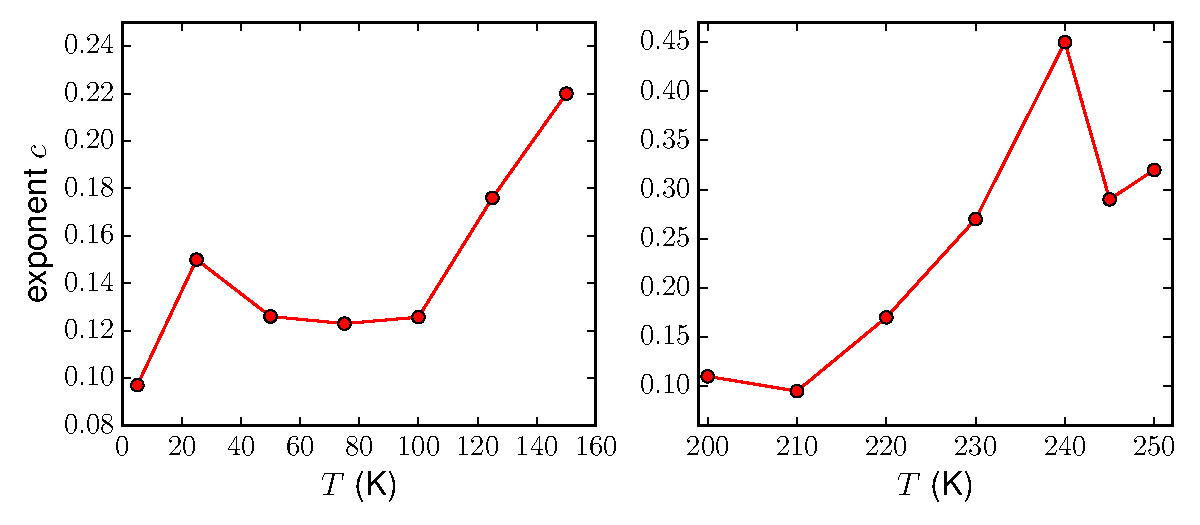
\includegraphics[width=0.7\columnwidth]{Chapter-4/experimental_exponent.pdf}
\protect\caption{The power-law exponents from experiments. The left figure is for CoO2 sample, and the right one is for CoO4 sample. The exponent may depend on the temperature and specific materials.}
\label{fig:rfim-expexp} 
\end{figure}


To simulate this complex experimental system,  we need to make several simplifying approximations. First, we are interested in the aging phenomena in the AF layer, and therefore model only this layer. We assume that the magnetization state of the thin AF film does not vary through its thickness, so that it can be approximated by a two-dimensional (2d) square lattice of Ising spins. We consider the staggered AF order parameter, which is modeled by the ferromagnetic exchange interaction of each spin with its four nearest neighbors.  In the experiments,  an external magnetic field is applied to fix the ferromagnetic spins parallel to each other, but the external field has negligible effect on AF spins. Therefore, The dipolar spin-spin interactions and the interaction with the  external fields used in our experiments are negligible, and the aging behavior is dominated by the interaction and frustration at the interface which can be approximated by random local fields $h_i$ coupled to each spin. The exchange interaction with F layer is described by an uncorrelated quenched random field $h_i$ with a Gaussian distribution $\mathcal{N}(0,\sigma_{\text{rand}}^{2})$ of zero mean and width $\sigma_{{\rm rand}}$. 
In this approximation, the reversal of the magnetization of F utilized in our experiments to initiate aging is modeled by the reversal of the random field.

The direct comparison between experimental material and simulational system is described as follows. The freshly prepared sample is coarse-grained to a two dimensional (2D) RFIM with a random spin initialization.  To obtain a stable magnetic state, the samples are cooled from $T=300K$ at a rate of $4K$ per minute to  low temperatures of $5K \sim 150K$ for aging; while, in the simulation, a similar approach is taken to anneal the system slowly to a stable state from $T=10$ to a certain low temperature ($0.1<T<1.0$). In the experiment, the aging is captured by measuring the resistance changes with time under flipping external magnetic field $H$. The flipping field $H$ is to keep the system in a measurable aging state. In the simulation, the energy relaxation is measured with flipping random fields, i.e. changing the sign of the random fields.

The random field Ising model, for example, in a square lattice, is described by the Hamiltonian is
\begin{equation}\label{energy}
\mathcal{H}=-J\sum_{<i,j>}s_{i}s_{j}-\sum_{i=1}^{N=L^{2}}h_{i}s_{i}
\end{equation}
where the coupling constant $J$ sets the overall energy scale and
is set to $1$ here, the spins are bimodal, $s_{i}=\pm1$, where $
\langle i,j \rangle$
enumerates nearest-neighbor spins,  $L$ is the linear dimension of the 2D square lattice with the total number of spins $N=L^{2}$, and periodic boundary conditions. The effects of temperature are modeled by the sequential random flipping of spins with the probability $P=\exp(-\Delta E/T)$ where $\Delta E$ is the energy change if the flipping is committed. The time $t$ is measured in sweeps, where one sweep corresponds to $N$ random sequential update attempts.  

The experimental system and connection with random field Ising model has been described and discussed in this section. The next section covers more details of the simulation.


\section{Monte Carlo Simulation}
The general procedure of MC simulation in RFIM is similar to that in Chapter \ref{chap-afm}, but the most challenging part is to approximate the experimental system with a reasonable set of procedures and parameters. Different procedures are tested to simulate the experimental procedure, and the final procedure used in the simulation is shown in the end of this section. Meanwhile, a wide range of parameters are also tested to explore the dynamics and behaviors of the RFIM, and all the parameters tested are shown in Table \ref{table:rfim-paras}. 

\begin{table}[h!]
\begin{center}
\begin{tabular}{l | r}
Variables              & Parameters \\
\hline
Temperature $T$ 	& 	$0.1 \sim 1.0$   \\
Random Field $\sigma_\text{rand}$            &		 0.1, 0.3, 0.5, 1.0   \\
Annealing rate $r$          & 	1e-1, 1e-2, 1e-3, 1e-4, 1e-5   \\
System Size $N$ 	&	  $32^2$, $64^2$, $128^2$, $256^2$   \\
MC sweeps in each cycle  	&	  $2,000 \sim 50,000$   \\
\end{tabular}
\end{center}
\caption{Parameters tested in the simulations.}
\label{table:rfim-paras}
\end{table}

In the simulation, we first anneal the system to the aging temperature $T$ at a slow rate of $r=0.0001$ per Monte Carlo sweep, which is comparable to the cooling process in the experiment. After the annealing, the system stops evolving at some metastable state with spin domains (as shown in Fig. \ref{fig:rfim-baaneal}). The snapshots before and after annealing is shown in Fig. \ref{fig:rfim-baaneal}. Then we simulate the aging at a fixed aging $T$ ($0.1\le T \le 1.0$). In the aging process, we flip the random fields every 20,000 MC sweeps, which excites the system to a non-equilibrium state. The parameters used in the simulations are determined by exploring a wide range of each parameter (see Table \ref{table:rfim-paras}). For example, annealing rates $\left( 10^{-1} \le r \le 10^{-5}\right)$ are tested to make sure that a metastable state is reached, and slower annealing rates lead to no significant changes to the metastable state. Another important parameter is the random field standard deviation $\sigma_{\rm rand}$ where too small $\sigma_{\rm rand}$ leads to plain 2D Ising model with exponential relaxation, and too big $\sigma_{\rm rand}$ would dominate the spin behavior comparing to unit near-neighbor spin interactions. 

\begin{figure}
\centering 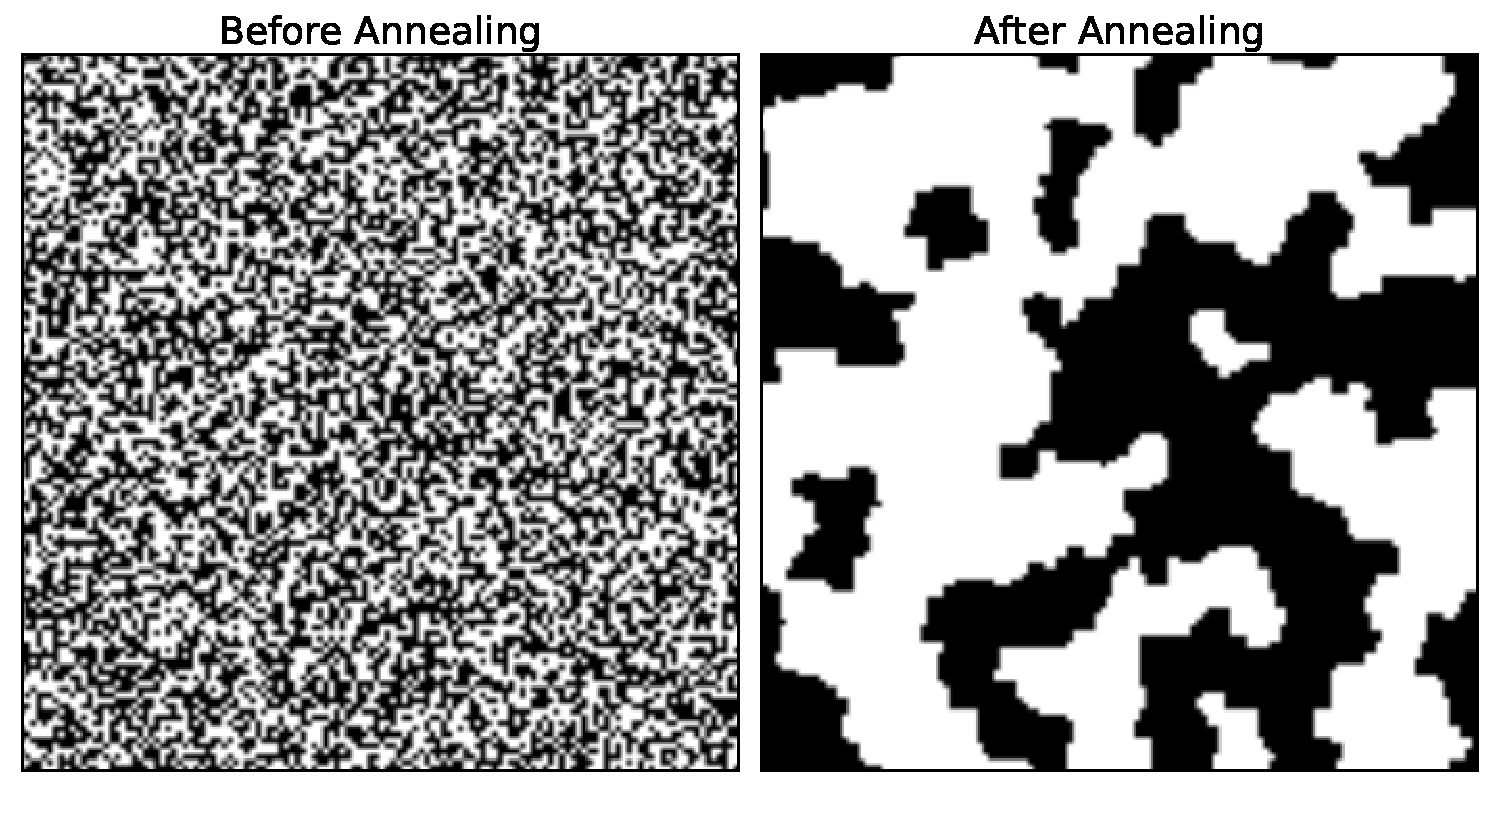
\includegraphics[width=0.9\columnwidth]{Chapter-4/RFIM_Before_After_Annealing}
\protect\caption{The snapshots of spin configurations before and after annealing of system size $L=128$. The state before annealing is simply a random state; while the state after annealing is a metastable state which seemingly does not change any more.}
\label{fig:rfim-baaneal} 
\end{figure}


After exploring different procedures and different parameters, the final procedure and parameters used in the simulation are
\begin{enumerate}
\item Randomly generate independent and identically distributed (i.i.d.) random field ($h_i\sim  \mathcal{N}(0, 1)$) and a random spin orientation ($s_i=\pm1$) for each site;
\item Anneal the system from temperature $T_0=10$ to the aging $T$ ($T=0.1\sim 0.5$) at a rate of $r=10^{-4}$, and the spins are randomly flipped using Metropolis choice based on the energy change;
\item After annealing to a certain temperature, fix the aging temperature $T$  ($T=0.1\sim 0.5$), flip the spins using Metropolis choice, and measure the energy relaxation;
\item Flip the random fields every $20,000$ MC sweeps after the annealing to keep the aging measurable in a reasonable time length.
\end{enumerate}

The results from simulation and their comparison to experiments are described in the next section below.


\section{Results and Comparison to Experiments}
\label{sec:rfim-results}
\begin{figure}
\centering 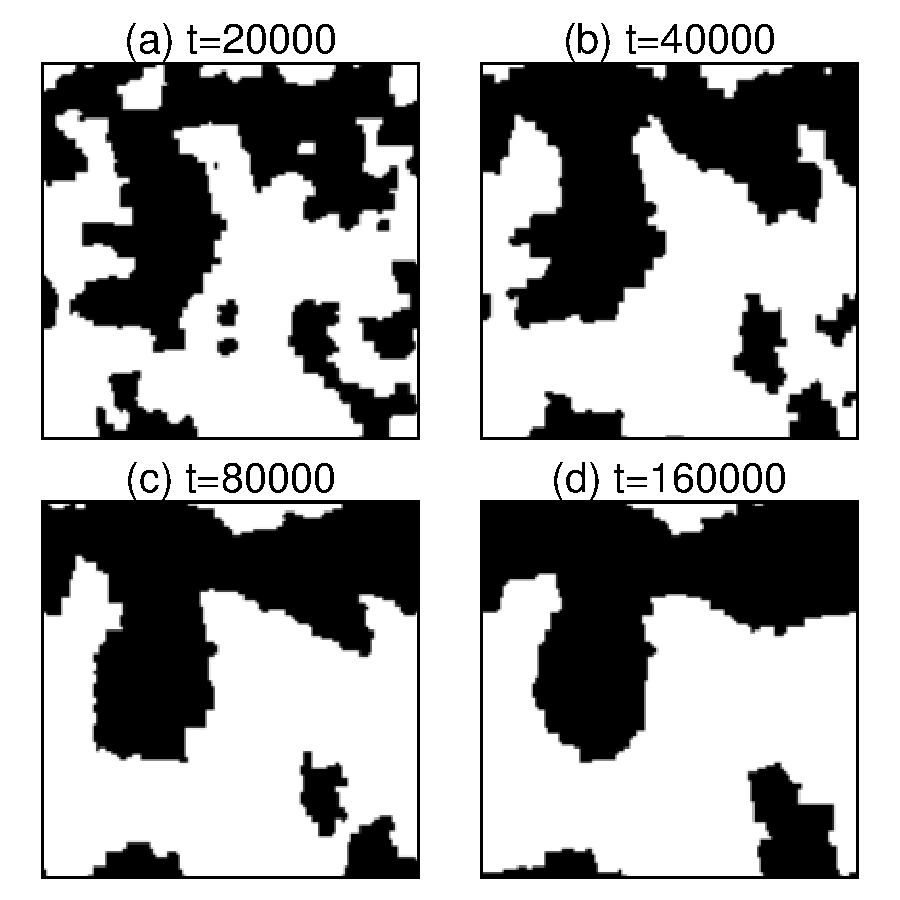
\includegraphics[width=0.8\columnwidth]{Chapter-4/spin_plot1_Norf}
\caption{Spin pattern snapshots in the Monte Carlo simulation at $T=0.3$ for the system size $L=128$. (a) is the spin pattern after the annealing and before the first random filed. (b), (c), and (d) are the spin snapshots at the end of cycles 1, 3, and 7, respectively. The corresponding energy changes can be found in Fig. \ref{fig:rfim-Es1}. In the aging process, there is clearly domain wall formed gradually. }
\label{fig:rfim-spinshots}
\end{figure}

\begin{figure}
\centering 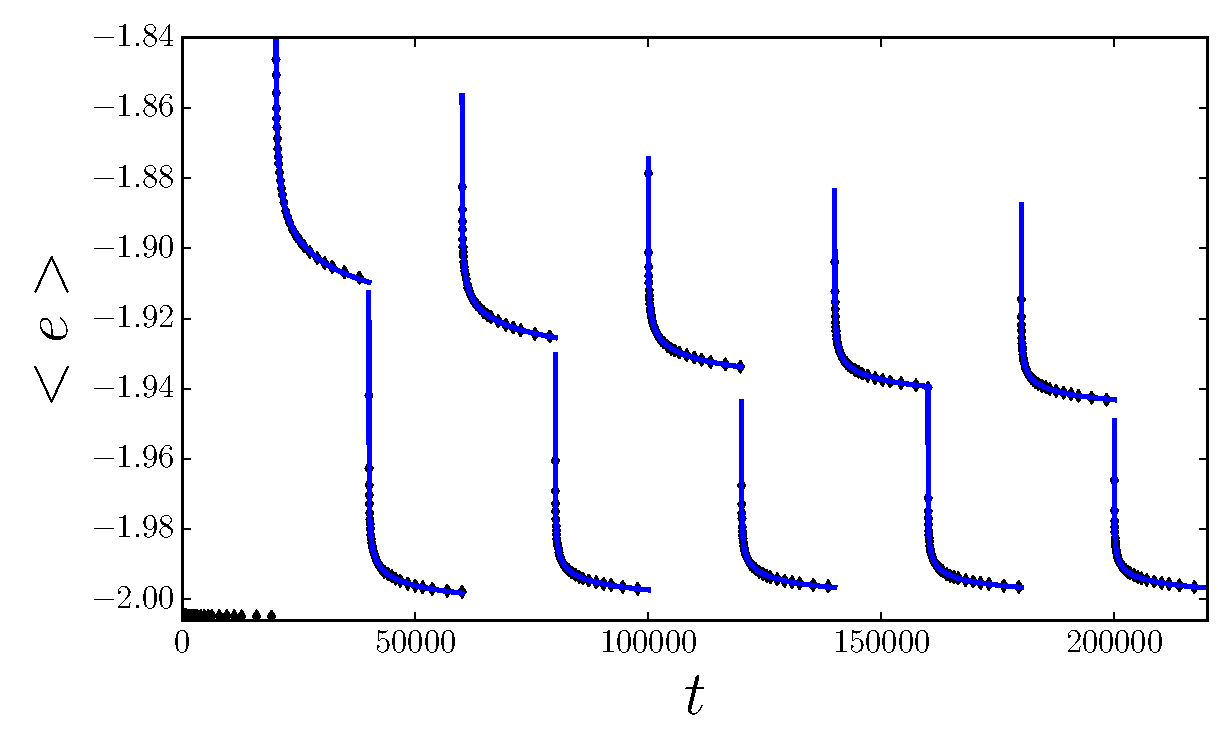
\includegraphics[width=0.8\columnwidth]{Chapter-4/Energy_simultion_fitted_10cycles_T03} 
\caption{Sequential simulations of energy relaxation for the system size $L=128$ with
random field $\sigma_{\text{rand}}=1.0$, temperature $T=0.3$. Black symbols represent an average of 100 simulation runs, and the blue curves are the power-law fittings with Eq.~(\ref{eq:rfim-fit}). Each individual simulation is performed starting with the initial state obtained by quasi-adiabatic annealing.}
\label{fig:rfim-Es1} 
\end{figure}

After the annealing, the system reaches a metastable state with interlocking spin domains of oppositely oriented spins. Although almost all spins are aligned with their neighbors at the end of annealing and attain their Ising-energy per spin, $\left\langle e\right\rangle \approx-2$,
see Fig.~\ref{fig:rfim-spinshots} and \ref{fig:rfim-Es1}, a sub-extensive amount of energy remains stored in rough domain walls that are pinned by the random field. To initiate aging at a fixed temperature $T$, we flip the random fields and simulate the evolution over 20,000 steps, after which the random field is flipped again and the simulations are repeated. The field flip brings the system into a non-equilibrium state, dislodging the domain walls. The snapshots of the spin distributions taken in the end of different aging cycles in Fig. \ref{fig:rfim-spinshots} show evolving spatial patterns, indicating that the system does  not relax to a unique equilibrium state, consistent with the experimental result \cite{ma2016prb}.

To establish the correlation with our experimental observations, a wide range of values (as shown in Table \ref{table:rfim-paras}) was explored for each parameter. For example, we tried the random field $\sigma_{\text{rand}}$ from $0.1 \sim 2.0$ where we found that small random fields would behave similarly as 2D Ising model, and big random fields would be dominate comparing to $J$. The measured variations of magneto-resistance due to aging are directly proportional to the variations of the local random field exerted by AF on F.  

\begin{figure}
\centering 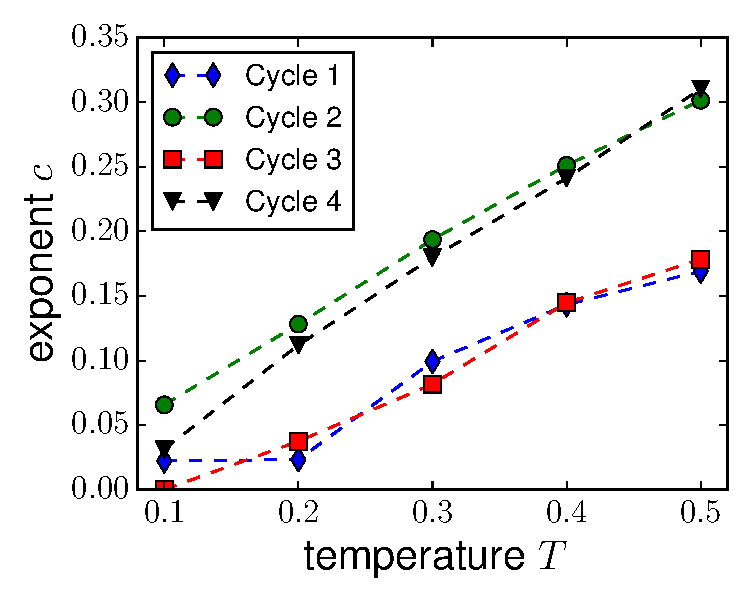
\includegraphics[width=0.5\columnwidth]{Chapter-4/exponent_scale_4cycle_T03}
\protect\caption{Dependence of exponent $c$ on temperature, for the system size $L=128$ with random field $\sigma_{\text{rand}}=1.0$. At low temperatures, the power-law fitting may not converge sometimes, for example, in Cycle 3 at $T=0.1$. That is also why no temperatures $T<0.1$ is used in the simulations. }
\label{fig:rfim-expT} 
\end{figure}

\begin{figure}
\centering 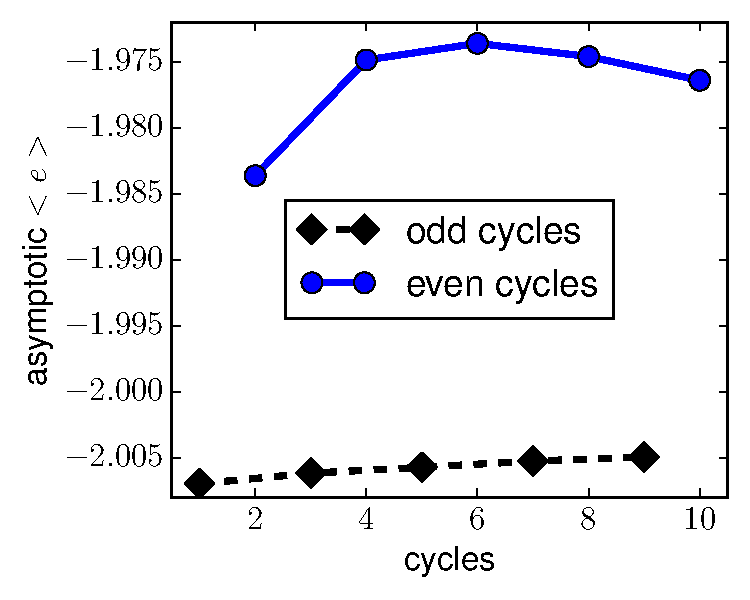
\includegraphics[width=0.5\columnwidth]{Chapter-4/asymptotic_E_T03_10cycles}
\protect\caption{Asymptotic energy for different aging cycles for system size $N=128^2$ at temperature $T=0.3$. The asymptotic energy is obtained from the power-law fitting at $t\rightarrow\infty$, i.e. $e_0$ in Eq \ref{eq:rfim-fit}. Other temperatures tested show the same pattern.} 
\label{fig:rfim-asm}
\end{figure}

To compare the results of our simulations to the experimental observations, we analyzed the evolution of the average
energy per spin $\langle e \rangle$ . We argue that the functional form of the time dependence of $\langle e \rangle$ is likely the same as that of the measured magneto-resistance, since the latter is directly proportional to the Zeeman energy of the ferromagnet, and other contributions to the energy of the F/AF system may be expected to evolve in a similar manner. An example of the time dependence of $\langle e \rangle$ including ten sequential aging cycles, starting from an annealed state, is shown in Fig. \ref{fig:rfim-Es1}. The obtained dependencies can be well described by the power law
\begin{equation}
e(t)=e_{0}+A\cdot  t^{-c}
\label{eq:rfim-fit}
\end{equation}
where $e_{0}$ is the asymptotic (equilibrium) energy, $A$ and $c$ are the scale and the exponent, respectively, and time $t$ is the number of the Monte Carlo sweep. We note that  changing the time scale in Eq.~\ref{eq:rfim-fit} simply rescales the value of $A$ without any effect on the exponent $c$, allowing direct comparison with the experiment. 

Fig. \ref{fig:rfim-expT} shows that the values of exponent determined from the simulations are very close to those obtained in our experiments as shown in Fig. \ref{fig:rfim-expexp}. The simulations also reproduce the relatively slow increase of $c$ with increasing temperatures. This results is inconsistent with the Neel-Arrhenius model. For example, for $c \approx 0.05$ at $T=0.1$, this model would predict $c=1.7$ at $T=0.5$, a much larger increase than in Fig. \ref{fig:rfim-expT}. There is no aging on the meaningful timescale at zero temperature, as expected for the thermal relaxation of the system. Fig. \ref{fig:rfim-asm} shows the dependence of the asymptotic (equilibrium) energy value $e_0$ provides further evidence that the system does not relax to a unique equilibrium state, and thus cannot be described by the Neel-Arrhenius model.



\section{Summary and Conclusion}
The experimental findings in the AF/F CoO/Py polycrystalline bilayer films show glassy dynamics and power-law aging effects with subunity exponents. In order to understand the aging phenomena, the thin film material is approximated by the random field Ising model on the 2D square lattice where the disordered AF/F interaction is described by the uncorrelated quenched random fields.

The simulational procedure and parameters are tuned to reproduce the the experimental system. Specifically, firstly, a slow annealing process is used to reach a metastable state with interlocking spin domains (as shown in Fig. \ref{fig:rfim-spinshots}); secondly, a set of parameters are tested to balance with random effects, finite size scaling, and computational cost; lastly, the energy states are recorded and compared to the resistance in experiments.

From the simulational results, the energy relaxation with respect to time is analyzed to compare to the experiments. A similar pattern to the experimental findings is observed. The power-law aging and subunity exponents $c$ are found, which can be directly compared to the results in the experiments. In addition to the small exponents, the asymptotic (equilibrium) energy values indicate that the system does not relax to a unique equilibrium state which may be the ground state at the low temperatures. Considering the power-law scaling, small exponents, and non-unique equilibrium state, the simulation also shows non-Neel-Arrhenius model.

In summary, the model used in the simulation simplifies the complex experimental system to only incorporate the two well-defined interactions: the nearest-neighbor exchange interaction, and the effective random fields produced by the interactions between the F/AF layers. Using a proper set of parameters and procedure, the Monte Carlo simulation reproduces the power-law aging and subunity exponents with non-unique equilibrium energies. The agreements between the experiment and the simulation provides a strong evidence for the dominance of frustration caused by the random exchange interaction at the F/AF interface, and may contribute insights to explain and understand other frustrated magnetic systems.

  





